\documentclass[11pt]{article}
\usepackage{hyperref}
\usepackage[english]{babel}
\usepackage{blindtext}
\usepackage{url}
\usepackage{graphicx}
\usepackage{multicol}
\usepackage[center]{titlesec}
\usepackage{geometry}
\usepackage{lettrine} % The lettrine is the first enlarged letter at the beginning of the text

%\usepackage{mathtools}

\usepackage[sort, numbers]{natbib}


%
%\setlength{\columnseprule}{0.4pt}
%\setlength{\footskip}{20pt}
\usepackage{fancyhdr}
\fancyhf{}
\fancyhead[C]{PHC 6016 $\bullet$ Joe Brew $\bullet$ Social Epidemiology}
\fancyfoot[C]{  $\bullet$ joebrew@gmail.com \bullet$  }
\renewcommand\headrulewidth{1pt}
\renewcommand\footrulewidth{1pt}
\pagestyle{fancy}

%

\setlength{\columnsep}{1.5cm}
%\setlength{\columnseprule}{0.4pt}

%\MakeOuterQuote{"}



\graphicspath{ {/home/joebrew/Documents/uf/phc6016/assignment6/assignment6_brew} }

%the next two lines adjust the third, centered section of the exec sum
\def\changemargin#1#2{\list{}{\rightmargin#2\leftmargin#1}\item[]}
\let\endchangemargin=\endlist 

\usepackage{Sweave}
\begin{document}
\Sconcordance{concordance:assignment6_brew.tex:assignment6_brew.Rnw:%
1 42 1 1 0 132 1}


\title{\textbf{Syndemic Approach to Childhood Obesity}}
\author{Joe Brew}


\maketitle

\noindent
Using an ecological or Syndemic approach, consider what other problems/epidemics may act synergistically with the problem you have chosen.  
In addition, carefully describe the potential relationships between the problems.
\begin{enumerate}
\item Co-occurring by chance;
\item Causing or predisposing to the other;
\item  All being caused by something else;
\item Being part of the same problem.
\end{enumerate}


\tableofcontents

\vspace{20mm}

\begin{center}

\includegraphics[width=2cm]{uf}
\end{center}


\newgeometry{margin=2.5cm}
%\fancyhfoffset[E,O]{0pt}


%------------------------------------------
\section*{Syndemicity, place and childhood obesity: an overview}
\addcontentsline{toc}{section}{Syndemicity, place and childhood obesity: an overview}
%------------------------------------------
\hrulefill

\begin{multicols}{2} 
\setkeys{Gin}{width=0.45\textwidth}

%------------------------------------------
\subsection*{Background}
\addcontentsline{toc}{subsection}{Background}
%------------------------------------------

\lettrine[nindent=0em,lines=3]{T}{he physiological causes of obesity}  in children are straighfroward, and can be simplified to a rudimentary thermodynamic equation:
\begin{center}
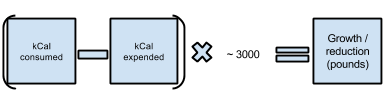
\includegraphics[width=6cm]{formula}
\end{center}

However, the relationship between calories consumed and calories expended is both mediated and confounded by numerous social factors with differential effect (in both magnitude and direction) by place, race, policies, socieoconomic status and culture.  Additionally, the purely thermodynamic understanding of obesity ignores a growing body of research highlighting metabolic differences across individuals, and even within the same individual as a result of environmental exposures and stress.\cite{Lee2014} Given the multicausal nature of the phenomenon of childhood obesity, some authors have begun referring to it as a "syndemic" rather than a "pandemic."\cite{Myslobodsky2010}  \\

This paper considers the problem of childhood obesity from a syndemic perspective, attempting to elucidate both how distal causes impact the thermodynamic equation, as well as how those distal causes interact with one another.  For the purposes of simplicity and brevity, I cover only five areas: place (geography), race (and/or ethnicity), socioeconomic status (SES), stress and culture.  
 

%------------------------------------------
\subsection*{Place}
\addcontentsline{toc}{subsection}{Place}
%------------------------------------------
The relationship between geography and adiposity has been well documented, and appears to be causal.\cite{vonHippel2014}  In the most immediate sense, one's place of residence carries with it environmental advantages and hazards pertaining both to the consumption and expenditure of calories as well as the lesser known obesity-related factors (such as chemical exposure).  In a looser sense, geography can affect adiposity in that geographic factors facilitate and/or limit behaviors which have a direct effect on the aforementioned thermodynamic equation.  \\

%------------------------------------------
\subsection*{Race}
\addcontentsline{toc}{subsection}{Race}
%------------------------------------------
In a cursary analysis of data from local school health screenings\footnote{Paper available here: https://github.com/joebrew/fdoh/blob/master/public/obesity/obesityKeri.pdf?raw=true}, being black or multiracial appeared to be a significant risk factor for obesity \emph{even after} adjustment for poverty (as measured by the proxy variable of free/reduced lunch status)\cite{Brew2014} Though rudimentary (free/reduced lunch is an overly simplistic and faulty proxy for deprivation), more refined studies have found that (in the US context), being of minority race/ethnicity appears positively correlated to overweight.\cite{Li2014}

%------------------------------------------
\subsection*{SES}
\addcontentsline{toc}{subsection}{SES}
%------------------------------------------
In the United States, low socioeconomic status correlates with obesity across racial, geographic, and cultural lines.  Among youth, being poor is an extremely strong predictor for being obese\cite{Lawman2014} Worryingly, some studies suggest that the importance and effect of SES as a predictor for obesity's more proximal causes (poor nutrition and inactivity) is growing.\cite{Buchtal2014}    


%------------------------------------------
\subsection*{Stress}
\addcontentsline{toc}{subsection}{Sress}
%------------------------------------------
Lack of sleep is one of the main results of stress, and appears to be independently assocaited with obesity.\cite{Graef2014}  In addition to this, stress itself, particularly insofar as it is related to social hierarchy and subordination, causes weight gain among humans.\cite{Tamashiro2007}

%------------------------------------------
\subsection*{Culture}
\addcontentsline{toc}{subsection}{Culture}
%------------------------------------------
Culture's effect on obesity can be seen most clearly in weight gain among migrants to the United States.\cite{Tovar2012} But the effect is not limited to those who migrate; cultural contexts affect "decisions"\footnote{In quotes, since free will probably doesn't exist.} ranging from breastfeeding to exercise.\cite{Young2012} Cultural beliefs and practices, though interacting with more proximal causes of obesity, are important in understanding differential prevalences among racial/ethnic groups.\cite{Spraggins2011}

%------------------------------------------
\subsection*{Syndemicity}
\addcontentsline{toc}{subsection}{Syndemicity}
%------------------------------------------
Geography, race, SES, stress and culture all co-occur significantly (but not completely). \\

One can still draw nearly perfect lines separating racial groups in the "post-segregation" south\footnote{http://projects.nytimes.com/census/2010/explorer?hp}.  But the relationship between geography and race extends to the north as well: in my summer work at the Chicago Department of Public Health, I found striking similarities between poverty and race by census tract (below)\footnote{https://joebrew.shinyapps.io/cdph/}:

\begin{center}
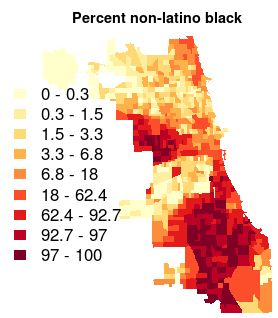
\includegraphics[width=3.5cm]{black} 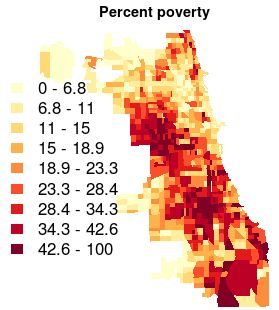
\includegraphics[width=3.5cm]{poverty}
\end{center}

Intuitively, geography can affect one's level of stress; but only recently have researchers begun to understand how factors like noise pollution trigger physiological responses.\cite{Chang2014}  \\

Intriguingly, though a great deal of attention goes to "food deserts" and access to nutrition, in the United States the relationship between place and adiposity appears to be mediated by physical activity, but \emph{not} mediated by diet.\cite{vonHippel2014} \\

No model fully describes the factors which mediate and confound the thermodynamic equation mentioned in the introduction; that said, the below diagram illustrates the five relationships between the five factors explained in this paper.
\begin{center}
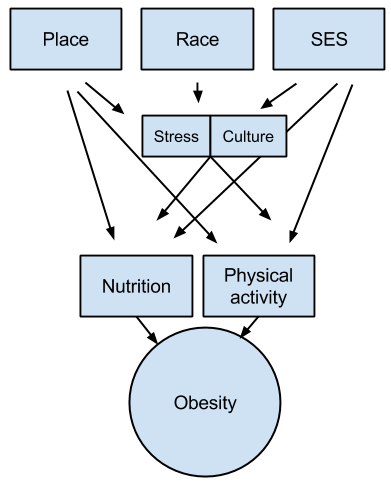
\includegraphics[width=7cm]{flow}
\end{center}


%------------------------------------------
\subsection*{Conclusion}
\addcontentsline{toc}{subsection}{Conclusion}
%------------------------------------------
Efforts to understand the obesity epidemic must be syndemic, in that they must take into account that an outcome (obesity) is not simply the sum of the causal factors, but rather the result of the many interactions between them.   Reductionist approaches to understanding (and thereby, addressing) the obesity epidemic have and will continue to fail.  "Targeted" interventions, though useful (and cost effective), will never address the underlying interactions that have lead to the highest prevalence of childhood obesity in history. The astounding number and complexity of causal interactions necessitate a syndemic framework to understand how we can reverse the trend.\cite{Fardet2014}







\end{multicols}
\setkeys{Gin}{width=1\textwidth}
%----------------------------------------------------------------------------------------
%  REFERENCE LIST
%----------------------------------------------------------------------------------------
%\newpage
\bibliographystyle{unsrtnat}
\bibliography{bibliography}


\end{document}
